\subsection{Occlusion Sensitivity Maps}
For testing occlusion sensitivity maps, we have used the model trained in the previous section. Results are given below. Note that the tuple in the caption is 
\[(\text{Size of occluder},\text{Stride of Occlusion})\]
Let us begin with looking at which areas of the image fire for classifying the image below as a wolf.
\begin{figure}[H]
    \centering
    \subfigure[]{
    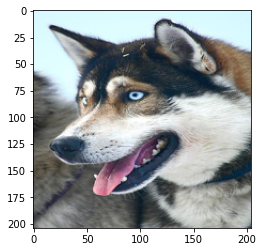
\includegraphics[width=.6\columnwidth]{occim1.png}}
    \qquad
    \subfigure[]{
    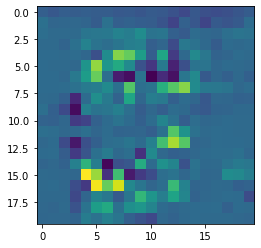
\includegraphics[width=.4\columnwidth]{occ1.png}}
    \qquad
    \subfigure[]{
    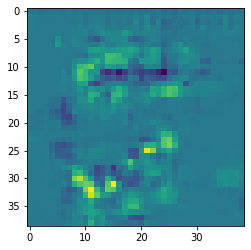
\includegraphics[width=.4\columnwidth]{occ1dash.png}}
    \caption[Short text]{Occlusion - (10,10) \& (10,5)}
\end{figure}
Let us look at another image of a dog with a man, and see which regions of the image indicate it is a dog.
\begin{figure}[H]
    \centering
    \subfigure[]{
    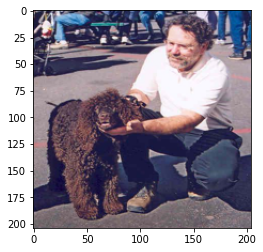
\includegraphics[width=.6\columnwidth]{occim2.png}}
    \qquad
    \subfigure[]{
    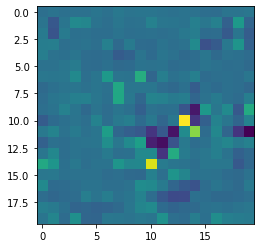
\includegraphics[width=.4\columnwidth]{occ2.png}}
    \qquad
    \subfigure[]{
    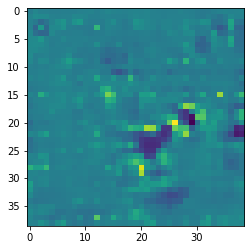
\includegraphics[width=.4\columnwidth]{occ2dash.png}}
    \caption[Short text]{Occlusion - (10,10) \& (10,5)}
\end{figure}
We can see that the model does not seem to be "looking" at the dog, and this is backed by the fact that probability of classification as a dog in this case is 67.96\%.